\documentclass[11pt]{article}
\usepackage{amsmath, amssymb, physics, mathtools, bm}
\usepackage{tikz, pgfplots}
\pgfplotsset{compat=1.18}
\usepackage[margin=2.3cm]{geometry}
\usepackage{siunitx, booktabs, hyperref}
\usepackage{braket}

\newcommand{\D}{\mathrm{D}}
\newcommand{\de}{\mathrm{d}}
\newcommand{\pd}[2]{\frac{\partial #1}{\partial #2}}
\newcommand{\pdd}[2]{\frac{\partial^{2} #1}{\partial #2^{2}}}
\newcommand{\Lap}{\nabla^{2}}

\title{B3: Quantum, Atomic and Molecular Physics --- Model Solutions, 2018}
\author{}
\date{}

\begin{document}
\maketitle

%==================================================================
\section*{Question 1 --- Fine structure of hydrogenic systems}

\subsection*{(a) Origin of fine structure and derivation of $\Delta E_\text{so}$}

\textbf{Problem.} Explain the physical origin of fine structure in hydrogenic atoms; derive $\Delta E_\text{so}=\tfrac{\beta}{2}[j(j+1)-l(l+1)-s(s+1)]$ and find $\beta$.

Physical origin: in the electron rest frame the proton orbits, generating a magnetic field $\vb B$; the electron spin magnetic moment $\bm\mu_s=-g_s\mu_B\vb S/\hbar$ couples to $\vb B$, giving the spin--orbit interaction (a relativistic correction of order $\alpha^2$).

Spin--orbit Hamiltonian (Thomas-corrected):
\[
H_\text{so} = \frac{1}{2m_e^2 c^2}\,\frac{1}{r}\frac{\de V}{\de r}\,\vb L\cdot\vb S,
\qquad V(r) = -\frac{Ze^2}{4\pi\epsilon_0 r}.
\]
Differentiate $V$:
\[
\frac{\de V}{\de r} = \frac{Ze^2}{4\pi\epsilon_0}\,\frac{1}{r^2}.
\]
Divide by $r$:
\[
\frac{1}{r}\frac{\de V}{\de r} = \frac{Ze^2}{4\pi\epsilon_0}\,\frac{1}{r^3}.
\]
Define $\xi(r)=(2m_e^2 c^2)^{-1}(1/r)(\de V/\de r)$:
\[
H_\text{so} = \xi(r)\,\vb L\cdot\vb S.
\]
Use $\vb J=\vb L+\vb S$:
\[
\vb J^2 = \vb L^2 + \vb S^2 + 2\vb L\cdot\vb S.
\]
Solve for $\vb L\cdot\vb S$:
\[
\vb L\cdot\vb S = \tfrac{1}{2}\bigl(\vb J^2 - \vb L^2 - \vb S^2\bigr).
\]
Take eigenvalues in $\ket{n\,l\,s\,j\,m_j}$:
\[
\langle\vb L\cdot\vb S\rangle = \tfrac{\hbar^2}{2}\bigl[j(j+1)-l(l+1)-s(s+1)\bigr].
\]
Take the radial expectation:
\[
\Delta E_\text{so} = \langle\xi(r)\rangle\,\tfrac{\hbar^2}{2}\bigl[j(j+1)-l(l+1)-s(s+1)\bigr].
\]
Identify $\beta = \hbar^2\langle\xi(r)\rangle$:
\[
\beta = \frac{\hbar^2}{2m_e^2 c^2}\,\frac{Ze^2}{4\pi\epsilon_0}\,\left\langle\frac{1}{r^3}\right\rangle.
\]
Insert the hint for $\langle 1/r^3\rangle$:
\[
\beta = \frac{\hbar^2}{2m_e^2 c^2}\,\frac{Ze^2}{4\pi\epsilon_0}\,\Bigl(\frac{Z}{na_0}\Bigr)^3\frac{1}{l(l+\tfrac12)(l+1)}.
\]
Collect powers of $Z$:
\[
\beta = \frac{\hbar^2 Z^4 e^2}{8\pi\epsilon_0 m_e^2 c^2\, n^3 a_0^3\, l(l+\tfrac12)(l+1)}.
\]
Substitute $a_0=4\pi\epsilon_0\hbar^2/(m_e e^2)$:
\[
a_0^3 = \frac{(4\pi\epsilon_0)^3\hbar^6}{m_e^3 e^6}.
\]
Insert into $\beta$:
\[
\beta = \frac{\hbar^2 Z^4 e^2}{8\pi\epsilon_0 m_e^2 c^2\, n^3 l(l+\tfrac12)(l+1)}\cdot\frac{m_e^3 e^6}{(4\pi\epsilon_0)^3\hbar^6}.
\]
Collect factors:
\[
\beta = \frac{Z^4 m_e e^8}{2(4\pi\epsilon_0)^4\hbar^4 c^2\, n^3 l(l+\tfrac12)(l+1)}.
\]
Identify $\alpha=e^2/(4\pi\epsilon_0\hbar c)$:
\[
\alpha^4 = \frac{e^8}{(4\pi\epsilon_0)^4\hbar^4 c^4}.
\]
Multiply top and bottom by $c^2$:
\[
m_e\cdot\frac{e^8}{(4\pi\epsilon_0)^4\hbar^4 c^2} = m_e c^2\cdot\frac{e^8}{(4\pi\epsilon_0)^4\hbar^4 c^4}.
\]
Identify the right-hand factor as $\alpha^4$:
\[
m_e\cdot\frac{e^8}{(4\pi\epsilon_0)^4\hbar^4 c^2} = \alpha^4\,m_e c^2.
\]
Substitute and simplify:
\[
\boxed{\;\beta = \frac{Z^4\alpha^4\, m_e c^2}{2 n^3 l(l+\tfrac12)(l+1)}\;}
\]
(equivalently $\beta = -E_n\,Z^2\alpha^2/[n\,l(l+\tfrac12)(l+1)]$ with $E_n=-\tfrac{1}{2}m_ec^2 Z^2\alpha^2/n^2$).

\subsection*{(b) Fine structure of $n=2,3$ in He$^+$}

He$^+$: $Z=2$, $s=1/2$. Combine $\Delta E_{\text{so}}=(\beta/2)[\dots]$ with $\beta$ from (a):
\[
\Delta E_\text{so} = \frac{Z^4 m_e c^2\alpha^4}{4 n^3\,l(l+\tfrac12)(l+1)}\,\bigl[j(j+1)-l(l+1)-s(s+1)\bigr].
\]
Evaluate $\alpha^4$ with $\alpha=1/137.036$:
\[
\alpha^4 = (1/137.036)^4 = 2.834\times 10^{-9}.
\]
Multiply by $m_ec^2=\SI{0.5110e6}{eV}$:
\[
m_e c^2\alpha^4 = \SI{0.5110e6}{eV}\times 2.834\times 10^{-9} = \SI{1.449}{meV}.
\]

\medskip
$n=2$: levels $2s_{1/2}$, $2p_{1/2}$, $2p_{3/2}$.
\begin{itemize}
\item $2s_{1/2}$: $l=0$ (no SO shift; included for completeness).
\item $2p_{1/2}$: $l=1,\;s=1/2,\;j=1/2$.

Compute the angular bracket:
\[
j(j+1)-l(l+1)-s(s+1) = \tfrac{3}{4}-2-\tfrac{3}{4} = -2.
\]
Compute the orbital denominator:
\[
l(l+\tfrac12)(l+1) = 1\cdot\tfrac32\cdot 2 = 3.
\]
Insert into $\Delta E_\text{so}$ with $Z^4=16$, $n^3=8$:
\[
\Delta E(2p_{1/2}) = \frac{16}{4\cdot 8\cdot 3}\cdot(-2)\cdot\SI{1.449}{meV}.
\]
Simplify the prefactor:
\[
\Delta E(2p_{1/2}) = -\tfrac{1}{3}\cdot\SI{1.449}{meV} = -\SI{0.483}{meV}.
\]
\item $2p_{3/2}$: $l=1,\;s=1/2,\;j=3/2$.

Compute the angular bracket:
\[
j(j+1)-l(l+1)-s(s+1) = \tfrac{15}{4}-2-\tfrac{3}{4} = +1.
\]
Insert into $\Delta E_\text{so}$:
\[
\Delta E(2p_{3/2}) = \frac{16}{4\cdot 8\cdot 3}\cdot(+1)\cdot\SI{1.449}{meV} = +\SI{0.242}{meV}.
\]
\end{itemize}

$n=3$: levels $3s_{1/2},\,3p_{1/2},\,3p_{3/2},\,3d_{3/2},\,3d_{5/2}$.

Compute overall prefactor for $n=3$, $Z=2$:
\[
\frac{Z^4 m_ec^2\alpha^4}{4n^3} = \frac{16}{4\cdot 27}\cdot\SI{1.449}{meV}.
\]
Simplify:
\[
\frac{Z^4 m_ec^2\alpha^4}{4n^3} = \frac{16}{108}\cdot\SI{1.449}{meV} = \SI{0.2147}{meV}.
\]
Compute angular ratios $[j(j+1)-l(l+1)-s(s+1)]/[l(l+\tfrac12)(l+1)]$:
\[
3p_{1/2}:\;\frac{-2}{3},\quad 3p_{3/2}:\;\frac{1}{3},
\]
\[
3d_{3/2}:\;\frac{-3}{15}=-\frac{1}{5},\quad 3d_{5/2}:\;\frac{2}{15}.
\]
Multiply each ratio by \SI{0.2147}{meV}:
\[
\Delta E(3p_{1/2}) = -\tfrac{2}{3}\cdot 0.2147\;\text{meV} = -\SI{0.143}{meV},
\]
\[
\Delta E(3p_{3/2}) = +\tfrac{1}{3}\cdot 0.2147\;\text{meV} = +\SI{0.0716}{meV},
\]
\[
\Delta E(3d_{3/2}) = -\tfrac{1}{5}\cdot 0.2147\;\text{meV} = -\SI{0.0429}{meV},
\]
\[
\Delta E(3d_{5/2}) = +\tfrac{2}{15}\cdot 0.2147\;\text{meV} = +\SI{0.0286}{meV}.
\]

\textit{Energy-level diagram:}
\begin{center}
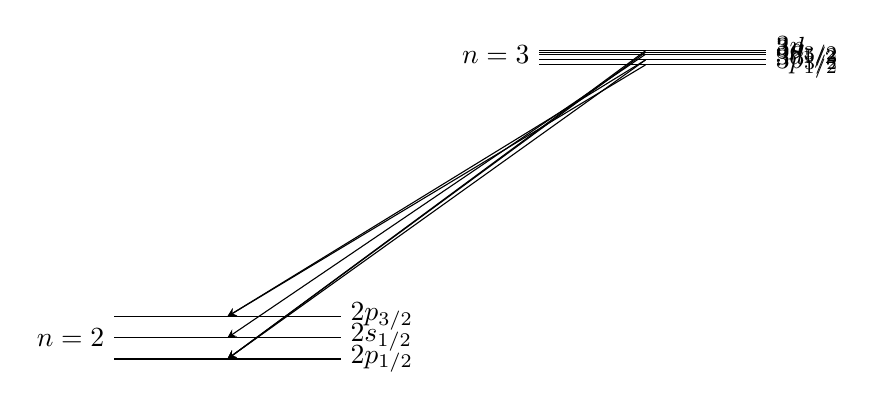
\begin{tikzpicture}[>=stealth, scale=0.9]
\draw (0,0) -- (3.2,0) node[right] {$2s_{1/2}$};
\draw (0,-0.3) -- (3.2,-0.3) node[right] {$2p_{1/2}$};
\draw (0,0.3) -- (3.2,0.3) node[right] {$2p_{3/2}$};
\node[left] at (0,0) {$n=2$};
\draw (6,4) -- (9.2,4) node[right] {$3s_{1/2}$};
\draw (6,3.85) -- (9.2,3.85) node[right] {$3p_{1/2}$};
\draw (6,4.05) -- (9.2,4.05) node[right] {$3p_{3/2}$};
\draw (6,3.92) -- (9.2,3.92) node[right] {$3d_{3/2}$};
\draw (6,4.03) -- (9.2,4.03) node[right] {$3d_{5/2}$};
\node[left] at (6,4) {$n=3$};
\draw[->] (7.5,3.85) -- (1.6,0.3);
\draw[->] (7.5,4.05) -- (1.6,-0.3);
\draw[->] (7.5,3.92) -- (1.6,-0.3);
\draw[->] (7.5,4.03) -- (1.6,-0.3);
\draw[->] (7.5,3.92) -- (1.6,0.3);
\draw[->] (7.5,4.0) -- (1.6,0);
\end{tikzpicture}
\end{center}

Allowed transitions ($\Delta l=\pm 1$, $\Delta j=0,\pm 1$, $j=0\not\to 0$):
\[
3p_{1/2}\!\to\!2s_{1/2},\;
3p_{3/2}\!\to\!2s_{1/2},\;
3s_{1/2}\!\to\!2p_{1/2},\;
3s_{1/2}\!\to\!2p_{3/2},
\]
\[
3d_{3/2}\!\to\!2p_{1/2},\;
3d_{3/2}\!\to\!2p_{3/2},\;
3d_{5/2}\!\to\!2p_{3/2}.
\]

\subsection*{(c) $\Omega^-$ bound to bare Pb (Z=82), $n=10$, $l=9$}

Splitting into 4 levels means $2s+1=4$:
\[
\boxed{\;s_\Omega = 3/2\;}
\]
Possible $j$ values $j=l-s,\dots,l+s$:
\[
j = 15/2,\;17/2,\;19/2,\;21/2.
\]

Reduced-mass effect: replace $m_e\to\mu = m_\Omega m_\text{Pb}/(m_\Omega+m_\text{Pb})\approx m_\Omega$ since the Pb nucleus is much heavier. Apply formula from (a) with $m_e\to m_\Omega$:
\[
\beta = \frac{Z^4\alpha^4 m_\Omega c^2}{2 n^3 l(l+\tfrac12)(l+1)}.
\]
Evaluate $Z^4$:
\[
Z^4 = 82^4 = \num{4.5212e7}.
\]
Evaluate $\alpha^4$:
\[
\alpha^4 = (1/137.036)^4 = \num{2.834e-9}.
\]
Multiply:
\[
Z^4\alpha^4 = 0.1281.
\]
Evaluate angular denominator $l(l+\tfrac12)(l+1)$:
\[
9\cdot 9.5\cdot 10 = 855.
\]
Combine with $n^3 = 1000$:
\[
\frac{Z^4\alpha^4}{2 n^3 l(l+\tfrac12)(l+1)} = \frac{0.1281}{2\cdot 1000\cdot 855} = \num{7.49e-8}.
\]
Multiply by $m_\Omega c^2 = \SI{1.672e9}{eV}$:
\[
\beta = \num{7.49e-8}\times\SI{1.672e9}{eV} = \SI{125.2}{eV}.
\]
Write the energy of level $j$:
\[
E_j = \tfrac{\beta}{2}\bigl[j(j+1)-l(l+1)-s(s+1)\bigr].
\]
Insert $l(l+1)=90$ and $s(s+1)=15/4$:
\[
E_j = \tfrac{\beta}{2}\bigl[j(j+1)-90-\tfrac{15}{4}\bigr].
\]
Take the difference $E_{j+1}-E_j$:
\[
E_{j+1}-E_j = \tfrac{\beta}{2}\bigl[(j+1)(j+2)-j(j+1)\bigr].
\]
Factor out $(j+1)$:
\[
(j+1)(j+2)-j(j+1) = (j+1)[(j+2)-j] = 2(j+1).
\]
Substitute back:
\[
E_{j+1}-E_j = \beta(j+1).
\]
Insert $j=15/2,17/2,19/2$:
\[
E_{17/2}-E_{15/2}=\tfrac{17}{2}\beta,\quad
E_{19/2}-E_{17/2}=\tfrac{19}{2}\beta,\quad
E_{21/2}-E_{19/2}=\tfrac{21}{2}\beta.
\]
Multiply by $\beta=\SI{125.2}{eV}$:
\[
\Delta E_{15/2\to 17/2} = \tfrac{17}{2}\cdot 125.2\;\text{eV} = \SI{1064}{eV},
\]
\[
\Delta E_{17/2\to 19/2} = \tfrac{19}{2}\cdot 125.2\;\text{eV} = \SI{1189}{eV},
\]
\[
\Delta E_{19/2\to 21/2} = \tfrac{21}{2}\cdot 125.2\;\text{eV} = \SI{1315}{eV}.
\]
Convert to keV:
\[
\boxed{\;\Delta E_{15/2\to 17/2} = \SI{1.06}{keV},\;\;
\Delta E_{17/2\to 19/2} = \SI{1.19}{keV},\;\;
\Delta E_{19/2\to 21/2} = \SI{1.31}{keV}.\;}
\]

\subsection*{(d) Two $\Omega^-$ bound to Pb: configurations $1s2l$ and ground}

The $\Omega^-$ has $s=3/2$ (half-integer), so it is a fermion. Pauli exclusion demands total wavefunction antisymmetric under exchange.

Couple two spin-$3/2$ particles:
\[
3/2\otimes 3/2 = 3\oplus 2\oplus 1\oplus 0.
\]
Identify exchange symmetry (standard result for two identical spin-$s$):
\begin{itemize}
\item $S=3,1$: spin symmetric;
\item $S=2,0$: spin antisymmetric.
\end{itemize}

\textit{Excited $1s\,2l$ configurations} ($l=0,1$): two particles in different spatial orbitals; spatial part can be either symmetric or antisymmetric.

For $1s\,2s$ ($L=0$), pair spatial $\pm$ with spin $\mp$:
\[
\text{spatial sym}\otimes\text{spin antisym}: \;{}^1S_0,\;{}^5S_2,
\]
\[
\text{spatial antisym}\otimes\text{spin sym}: \;{}^3S_1,\;{}^7S_3.
\]
Collect levels for $1s2s$:
\[
\boxed{\;{}^1S_0,\,{}^3S_1,\,{}^5S_2,\,{}^7S_3\;}.
\]

For $1s\,2p$ ($L=1$), repeat the pairing:
\[
\text{spatial sym}\otimes\text{spin antisym}: \;{}^1P_1,\;{}^5P_{1,2,3},
\]
\[
\text{spatial antisym}\otimes\text{spin sym}: \;{}^3P_{0,1,2},\;{}^7P_{2,3,4}.
\]
Collect levels for $1s2p$:
\[
\boxed{\;{}^1P_1,\;{}^3P_{0,1,2},\;{}^5P_{1,2,3},\;{}^7P_{2,3,4}\;}.
\]

\textit{Ground configuration $1s^2$}: both particles in the same spatial orbital, so spatial part is necessarily symmetric. Spin must therefore be antisymmetric:
\[
S=0,2 \;\Rightarrow\; \boxed{\;\text{ground: }{}^1S_0\;\text{and}\;{}^5S_2\;}.
\]

\textit{Comparison with He}: two spin-$1/2$ electrons in $1s^2$ admit only the antisymmetric singlet $S=0$, giving uniquely ${}^1S_0$. Two spin-$3/2$ $\Omega^-$ admit \emph{two} antisymmetric spin states ($S=0,2$), so the ground configuration contains both ${}^1S_0$ and ${}^5S_2$ --- a richer multiplet structure than helium.

%==================================================================
\section*{Question 2 --- Helium, Zeeman effect, positronium}

\subsection*{(a) He levels for $1s^2$, $1s2s$, $1s2p$}

Configurations and terms:
\begin{itemize}
\item $1s^2$: ${}^1S_0$ only (Pauli; spatial sym requires spin antisym).
\item $1s2s$: ${}^1S_0$, ${}^3S_1$.
\item $1s2p$: ${}^1P_1$, ${}^3P_{0,1,2}$.
\end{itemize}

\begin{center}
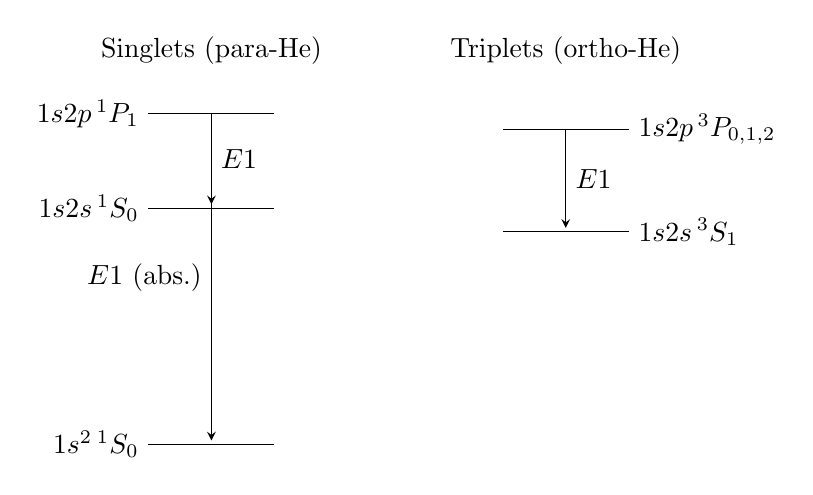
\begin{tikzpicture}[>=stealth, scale=1.0]
% singlets (left)
\draw (0,0) -- (1.6,0) node[left=22pt,below=0pt]{}; \node[left] at (0,0) {$1s^2\,{}^1S_0$};
\draw (0,3) -- (1.6,3); \node[left] at (0,3) {$1s2s\,{}^1S_0$};
\draw (0,4.2) -- (1.6,4.2); \node[left] at (0,4.2) {$1s2p\,{}^1P_1$};
% triplets (right)
\draw (4.5,2.7) -- (6.1,2.7); \node[right] at (6.1,2.7) {$1s2s\,{}^3S_1$};
\draw (4.5,4.0) -- (6.1,4.0); \node[right] at (6.1,4.0) {$1s2p\,{}^3P_{0,1,2}$};
% allowed E1 transitions
\draw[->] (0.8,4.2) -- (0.8,3.05) node[midway,right] {$E1$};
\draw[->] (0.8,4.2) -- (0.8,0.05) node[midway,left] {$E1$ (abs.)};
\draw[->] (5.3,4.0) -- (5.3,2.75) node[midway,right] {$E1$};
% labels
\node at (0.8,5) {Singlets (para-He)};
\node at (5.3,5) {Triplets (ortho-He)};
\end{tikzpicture}
\end{center}

Selection rules ($\Delta S=0$, $\Delta L=\pm 1$, $\Delta J=0,\pm 1$, $J=0\not\to 0$, parity changes):
allowed E1 transitions are $1s2p\,{}^1P_1\!\to\!1s^2\,{}^1S_0$, $1s2p\,{}^1P_1\!\to\!1s2s\,{}^1S_0$, and $1s2p\,{}^3P_{0,1,2}\!\to\!1s2s\,{}^3S_1$.

\textit{Absorption}: only from the ground state $1s^2\,{}^1S_0$, hence only $1s^2\,{}^1S_0\!\to\!1s2p\,{}^1P_1$.

\textit{Intercombination lines} (singlet-triplet): forbidden by $\Delta S=0$ to first order. He is light, so spin--orbit mixing is tiny; intercombination lines are very weak (the famous $1s2s\,{}^3S_1\!\to\!1s^2\,{}^1S_0$ is metastable). \textbf{Not} prominent.

\subsection*{(b) Weak-field Zeeman effect in $LS$ coupling}

Weak field: $H_\text{Zeeman}\ll H_\text{so}$, so $\vb J$ is a good quantum number; $\vb L$ and $\vb S$ precess about $\vb J$, while $\vb J$ precesses slowly about $\vb B$.

Write the Zeeman Hamiltonian:
\[
H_Z = \frac{\mu_B}{\hbar}(\vb L + g_s\vb S)\cdot\vb B,\qquad g_s\approx 2.
\]
Take $\vb B = B\hat{\vb z}$:
\[
H_Z = \frac{\mu_B B}{\hbar}(L_z + 2 S_z).
\]
Apply the projection theorem for $\vb V = \vb L + 2\vb S$ within an $\ket{LSJM_J}$ manifold:
\[
\langle\vb V\rangle = \frac{\langle\vb V\cdot\vb J\rangle}{\langle\vb J^2\rangle}\,\langle\vb J\rangle \equiv g_J\,\langle\vb J\rangle.
\]
Expand $\vb V\cdot\vb J = (\vb L+2\vb S)\cdot(\vb L+\vb S)$:
\[
\vb V\cdot\vb J = \vb L^2 + \vb L\cdot\vb S + 2\vb S\cdot\vb L + 2\vb S^2 = \vb L^2 + 3\,\vb L\cdot\vb S + 2\vb S^2.
\]
Solve $\vb J^2=\vb L^2+\vb S^2+2\vb L\cdot\vb S$ for $\vb L\cdot\vb S$:
\[
\vb L\cdot\vb S = \tfrac{1}{2}(\vb J^2 - \vb L^2 - \vb S^2).
\]
Substitute into $\vb V\cdot\vb J$:
\[
\vb V\cdot\vb J = \vb L^2 + \tfrac{3}{2}(\vb J^2 - \vb L^2 - \vb S^2) + 2\vb S^2.
\]
Collect terms:
\[
\vb V\cdot\vb J = \tfrac{3}{2}\vb J^2 - \tfrac{1}{2}\vb L^2 + \tfrac{1}{2}\vb S^2.
\]
Take expectation in $\ket{LSJM_J}$ and divide by $\langle\vb J^2\rangle=J(J+1)\hbar^2$:
\[
g_J = \frac{\tfrac{3}{2}J(J+1) - \tfrac{1}{2}L(L+1) + \tfrac{1}{2}S(S+1)}{J(J+1)}.
\]
Rewrite $3/2 = 1 + 1/2$:
\[
g_J = 1 + \frac{J(J+1)+S(S+1)-L(L+1)}{2J(J+1)}.
\]
Energy shift in eigenstate $\ket{LSJM_J}$:
\[
\boxed{\;\Delta E_Z = g_J\,\mu_B B\,M_J,\quad M_J=-J,\dots,J.\;}
\]

\subsection*{(c) Zeeman patterns for the two transitions}

\textit{$1s3s\,{}^1S_0\!\to\!1s2p\,{}^1P_1$ (singlet)}: $S=0$ in both terms, so $g_J=1$ for both --- \textbf{normal Zeeman effect}.

Upper $J=0$: $M_J=0$ only, no splitting.
Lower $J=1$: $M_J=-1,0,+1$, shifts $-\mu_B B,\,0,\,+\mu_B B$.

Write the emission frequency for $u\to l$:
\[
\nu = \nu_0 + (g_u M_u - g_l M_l)\mu_B B/h.
\]
Set $g_u=g_l=1$ and $M_u=0$:
\[
\nu = \nu_0 - M_l\,\mu_B B/h.
\]
Insert $M_l=-1,0,+1$:
\[
\nu = \nu_0+\mu_B B/h,\quad \nu_0,\quad \nu_0-\mu_B B/h.
\]
Polarisations:
\begin{itemize}
\item $\Delta M_J = M_u-M_l = \pm 1$: $\sigma^\pm$ (circular along $\vb B$; linear $\perp\vb B$ transverse).
\item $\Delta M_J = 0$: $\pi$ (linear $\parallel\vb B$; visible only in transverse observation).
\end{itemize}

\textit{$1s3s\,{}^3S_1\!\to\!1s2p\,{}^3P_1$ (triplet)}: \textbf{anomalous Zeeman effect}.

Compute Landé for upper ${}^3S_1$ ($L=0,S=1,J=1$):
\[
g({}^3S_1) = 1+\frac{1\cdot 2+1\cdot 2-0}{2\cdot 1\cdot 2} = 1+\frac{4}{4} = 2.
\]
Compute Landé for lower ${}^3P_1$ ($L=1,S=1,J=1$):
\[
g({}^3P_1) = 1+\frac{1\cdot 2+1\cdot 2-1\cdot 2}{2\cdot 1\cdot 2} = 1+\frac{2}{4} = \tfrac{3}{2}.
\]
Sub-level shifts in units of $\mu_B B$: upper $\{-2,0,+2\}$; lower $\{-3/2,0,+3/2\}$.

Write the emission frequency:
\[
\nu = \nu_0 + (g_u M_u - g_l M_l)\mu_B B/h = \nu_0 + (2 M_u - \tfrac{3}{2}M_l)\mu_B B/h.
\]
Apply selection rules $\Delta M=0,\pm 1$ with $M=0\not\to M=0$ for $\Delta J=0$.

Enumerate $\sigma^+$ ($M_u-M_l=+1$): $(M_u,M_l)=(+1,0)$ and $(0,-1)$:
\[
(2\cdot 1 - 0) = +2,\qquad (0 - \tfrac{3}{2}(-1)) = +\tfrac{3}{2}.
\]
Enumerate $\sigma^-$ ($M_u-M_l=-1$): $(M_u,M_l)=(-1,0)$ and $(0,+1)$:
\[
(2\cdot(-1)-0) = -2,\qquad (0-\tfrac{3}{2}\cdot 1) = -\tfrac{3}{2}.
\]
Enumerate allowed $\pi$ ($\Delta M=0$, $M\ne 0$): $(M_u,M_l)=(\pm 1,\pm 1)$:
\[
(2-\tfrac{3}{2}) = +\tfrac{1}{2},\qquad (-2+\tfrac{3}{2}) = -\tfrac{1}{2}.
\]
Total: 4 $\sigma$ and 2 $\pi$ components, so 6 triplet lines.

\begin{center}
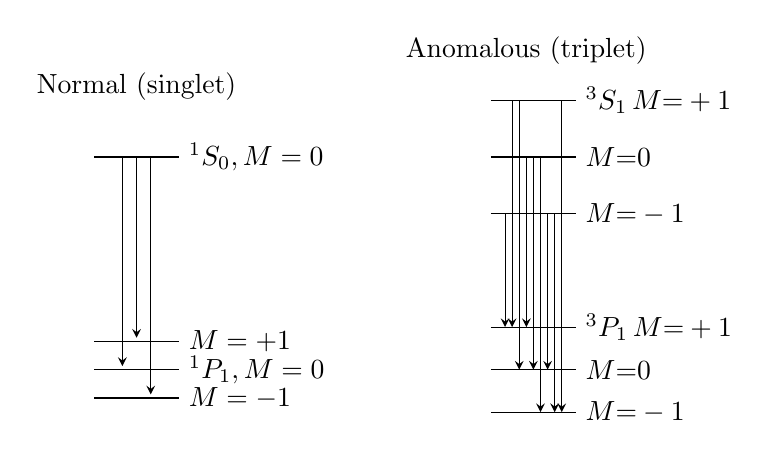
\begin{tikzpicture}[>=stealth, scale=0.9]
% normal Zeeman
\draw (-0.6,3) -- (0.6,3) node[right]{${}^1S_0,M=0$};
\draw (-0.6,0) -- (0.6,0) node[right]{${}^1P_1,M=0$};
\draw (-0.6,0.4) -- (0.6,0.4) node[right]{$M=+1$};
\draw (-0.6,-0.4) -- (0.6,-0.4) node[right]{$M=-1$};
\draw[->] (0,3) -- (0,0.45);
\draw[->] (-0.2,3) -- (-0.2,0.05);
\draw[->] (0.2,3) -- (0.2,-0.35);
\node at (0,4) {Normal (singlet)};
% anomalous Zeeman
\draw (5,3.8) -- (6.2,3.8) node[right]{${}^3S_1\,M{=}+1$};
\draw (5,3.0) -- (6.2,3.0) node[right]{$M{=}0$};
\draw (5,2.2) -- (6.2,2.2) node[right]{$M{=}-1$};
\draw (5,0.6) -- (6.2,0.6) node[right]{${}^3P_1\,M{=}+1$};
\draw (5,0.0) -- (6.2,0.0) node[right]{$M{=}0$};
\draw (5,-0.6) -- (6.2,-0.6) node[right]{$M{=}-1$};
\foreach \mu/\ml in {3.8/0.6,3.8/0.0,3.0/0.6,3.0/0.0,3.0/-0.6,2.2/0.0,2.2/-0.6,3.8/-9,2.2/0.6}{}
\draw[->] (5.3,3.8) -- (5.3,0.6);
\draw[->] (5.4,3.8) -- (5.4,0.0);
\draw[->] (5.5,3.0) -- (5.5,0.6);
\draw[->] (5.6,3.0) -- (5.6,0.0);
\draw[->] (5.7,3.0) -- (5.7,-0.6);
\draw[->] (5.8,2.2) -- (5.8,0.0);
\draw[->] (5.9,2.2) -- (5.9,-0.6);
\draw[->] (5.2,2.2) -- (5.2,0.6);
\draw[->] (6.0,3.8) -- (6.0,-0.6);
\node at (5.5,4.5) {Anomalous (triplet)};
\end{tikzpicture}
\end{center}

\subsection*{(d) Six lines $\Rightarrow$ orientation; minimum $B$}

Total components: triplet gives $4\sigma + 2\pi = 6$; singlet gives $2\sigma+1\pi=3$; total 9. Observing only 6 means all 3 $\pi$ components are absent. $\pi$-light has $\vb E\parallel\vb B$ and so radiates only transverse to $\vb B$; it vanishes in longitudinal observation. Conclude:
\[
\boxed{\;\text{Observer is along the magnetic field, }\vb k\parallel\vb B;\;\text{only }\sigma^\pm\text{ visible: }4+2=6\text{ lines.}\;}
\]

Write the pressure-broadened linewidth (FWHM):
\[
\Delta\nu = \frac{1}{2\pi\tau_\text{coll}},\qquad \tau_\text{coll}^{-1} = n\sigma\bar v,\qquad \sigma=\pi(2r)^2.
\]
Compute the number density from the ideal-gas law:
\[
n = \frac{P}{k_B T} = \frac{0.1}{1.381\times 10^{-23}\times 10}.
\]
Evaluate:
\[
n = \SI{7.24e20}{m^{-3}}.
\]
Write the Maxwell--Boltzmann mean speed:
\[
\bar v = \sqrt{\frac{8k_B T}{\pi m_\text{He}}}.
\]
Insert $m_\text{He}=4\times\SI{1.66e-27}{kg}=\SI{6.64e-27}{kg}$ and $T=\SI{10}{K}$:
\[
\bar v = \sqrt{\frac{8\cdot 1.381\times 10^{-23}\cdot 10}{\pi\cdot 6.64\times 10^{-27}}}.
\]
Simplify the radicand:
\[
\bar v = \sqrt{5.30\times 10^{4}\;\text{m}^2/\text{s}^2}.
\]
Evaluate:
\[
\bar v = \SI{230}{m/s}.
\]
Compute the hard-sphere cross-section with $r=\SI{0.1}{nm}$:
\[
\sigma = \pi(2r)^2 = \pi(0.2\times 10^{-9}\;\text{m})^2 = \SI{1.26e-19}{m^2}.
\]
Compute the collision rate:
\[
\tau_\text{coll}^{-1} = n\sigma\bar v = 7.24\times 10^{20}\cdot 1.26\times 10^{-19}\cdot 230.
\]
Evaluate:
\[
\tau_\text{coll}^{-1} = \SI{2.10e4}{s^{-1}}.
\]
Divide by $2\pi$ to get the linewidth:
\[
\Delta\nu = \frac{2.10\times 10^{4}}{2\pi} = \SI{3.34e3}{Hz}.
\]
List $\sigma$-shifts about each line centre (units $\mu_B B/h$): singlet $\{-1,+1\}$ and triplet $\{-2,-\tfrac{3}{2},+\tfrac{3}{2},+2\}$.

Identify the smallest adjacent gap (between triplet shifts $-2$ and $-3/2$, or between $+3/2$ and $+2$):
\[
\Delta\nu_\text{min} = \tfrac{1}{2}\,\mu_B B/h.
\]
Equate $\Delta\nu_\text{min}=\Delta\nu$ and solve for $B$:
\[
B_\text{min} = \frac{2 h\,\Delta\nu}{\mu_B}.
\]
Insert numbers:
\[
B_\text{min} = \frac{2\cdot 6.626\times 10^{-34}\cdot 3.34\times 10^{3}}{9.274\times 10^{-24}}.
\]
Evaluate the numerator:
\[
2\cdot 6.626\times 10^{-34}\cdot 3.34\times 10^{3} = 4.43\times 10^{-30}\;\text{J s Hz}.
\]
Divide by $\mu_B$:
\[
\boxed{\;B_\text{min}\approx\SI{4.8e-7}{T}\sim\SI{0.5}{\micro T}.\;}
\]

\subsection*{(e) Positronium ground configuration}

Electron and positron are both spin-$1/2$. Couple $1/2\otimes 1/2 = 0\oplus 1$:
\[
\boxed{\;S=0\;(\text{para-positronium, }{}^1S_0),\quad S=1\;(\text{ortho-positronium, }{}^3S_1).\;}
\]

Apply $\vb B = B\hat{\vb z}$. Electron moment $\bm\mu_{e^-}=-g_s\mu_B\vb S_{e^-}/\hbar$; positron has opposite-sign $g$-factor, so $\bm\mu_{e^+}=+g_s\mu_B\vb S_{e^+}/\hbar$.

Sum the moments:
\[
\bm\mu_{e^-}+\bm\mu_{e^+} = -\frac{g_s\mu_B}{\hbar}\bigl(\vb S_{e^-}-\vb S_{e^+}\bigr).
\]
Form the Zeeman Hamiltonian $H_Z=-(\bm\mu_{e^-}+\bm\mu_{e^+})\cdot\vb B$:
\[
H_Z = \frac{g_s\mu_B B}{\hbar}\bigl(S^{e^-}_z - S^{e^+}_z\bigr).
\]
Write the singlet and triplet $M=0$ kets:
\[
\ket{1,0} = \tfrac{1}{\sqrt 2}(\ket{\uparrow\downarrow}+\ket{\downarrow\uparrow}),\qquad
\ket{0,0} = \tfrac{1}{\sqrt 2}(\ket{\uparrow\downarrow}-\ket{\downarrow\uparrow}).
\]
Act with $S^{e^-}_z-S^{e^+}_z$ on each product ket:
\[
(S^{e^-}_z-S^{e^+}_z)\ket{\uparrow\downarrow} = \tfrac{\hbar}{2}\ket{\uparrow\downarrow} - (-\tfrac{\hbar}{2})\ket{\uparrow\downarrow} = \hbar\ket{\uparrow\downarrow},
\]
\[
(S^{e^-}_z-S^{e^+}_z)\ket{\downarrow\uparrow} = -\tfrac{\hbar}{2}\ket{\downarrow\uparrow} - \tfrac{\hbar}{2}\ket{\downarrow\uparrow} = -\hbar\ket{\downarrow\uparrow}.
\]
Apply to $\ket{1,0}$:
\[
(S^{e^-}_z-S^{e^+}_z)\ket{1,0} = \tfrac{\hbar}{\sqrt 2}(\ket{\uparrow\downarrow}-\ket{\downarrow\uparrow}) = \hbar\ket{0,0}.
\]
Take the inner product with $\bra{0,0}$:
\[
\bra{0,0}(S^{e^-}_z-S^{e^+}_z)\ket{1,0} = \hbar.
\]
Multiply by the prefactor of $H_Z$:
\[
\bra{0,0} H_Z \ket{1,0} = g_s\mu_B B.
\]
The triplet $M=\pm 1$ states $\ket{\uparrow\uparrow}$, $\ket{\downarrow\downarrow}$ satisfy $(S^{e^-}_z-S^{e^+}_z)\ket{\pm\pm}=0$, so they are unshifted to first order.

\textit{Effect}: the field \textbf{mixes the singlet $\ket{0,0}$ with the triplet $\ket{1,0}$} rather than producing the usual linear Zeeman splitting. The two extreme triplet sublevels $M=\pm 1$ are unshifted to leading order; the two $M=0$ states repel each other quadratically in $B$ (an avoided crossing). This is the textbook Breit--Rabi ortho--para mixing in positronium hyperfine spectroscopy.

%==================================================================
\section*{Question 3 --- Rabi oscillations and three-level dynamics}

\subsection*{(a) Meaning of $\Omega_R$}

Semiclassical dipole interaction: $H_\text{int}=-\bm{d}\cdot\vb E_0\cos\omega t$. Rabi frequency:
\[
\boxed{\;\Omega_R = \frac{|\!\bra{2}\bm{d}\cdot\hat{\bm\epsilon}\ket{1}\!|\,E_0}{\hbar}\;}
\]
\textbf{$\Omega_R$ is the on-resonance Rabi frequency} = oscillation frequency of population between $\ket{1}$ and $\ket{2}$ on resonance, set by the dipole matrix element times the field amplitude (in units of $\hbar$). Period $2\pi/\Omega_R$ corresponds to a $2\pi$ pulse.

\subsection*{(b) Rotating wave approximation; weak-light solution}

Write $\cos\omega t = (e^{i\omega t}+e^{-i\omega t})/2$ in $\dot c_2$:
\[
\dot c_2 = -i\tfrac{\Omega_R}{2}\bigl[e^{i(\omega_0+\omega)t} + e^{i(\omega_0-\omega)t}\bigr]c_1.
\]
RWA: drop the rapidly oscillating term $e^{i(\omega_0+\omega)t}$:
\[
\dot c_2 = -i\tfrac{\Omega_R}{2}\,e^{-i\delta\omega\, t} c_1,\qquad \delta\omega \equiv \omega-\omega_0.
\]
Similarly for $\dot c_1$:
\[
\dot c_1 = -i\tfrac{\Omega_R}{2}\,e^{i\delta\omega\, t} c_2.
\]
Differentiate the $\dot c_2$ equation:
\[
\ddot c_2 = -i\tfrac{\Omega_R}{2}\bigl[-i\delta\omega\, e^{-i\delta\omega t}c_1 + e^{-i\delta\omega t}\dot c_1\bigr].
\]
Identify $-i(\Omega_R/2)e^{-i\delta\omega t}c_1 = \dot c_2$:
\[
\ddot c_2 = -i\delta\omega\,\dot c_2 -i\tfrac{\Omega_R}{2}e^{-i\delta\omega t}\dot c_1.
\]
Substitute $\dot c_1 = -i(\Omega_R/2)e^{i\delta\omega t}c_2$:
\[
\ddot c_2 = -i\delta\omega\,\dot c_2 + (-i)^2\tfrac{\Omega_R^2}{4}e^{-i\delta\omega t}e^{i\delta\omega t}c_2.
\]
Cancel the exponentials and use $(-i)^2=-1$:
\[
\ddot c_2 = -i\delta\omega\,\dot c_2 - \tfrac{\Omega_R^2}{4}c_2.
\]
Rearrange to standard form:
\[
\ddot c_2 + i\delta\omega\,\dot c_2 + \tfrac{\Omega_R^2}{4}c_2 = 0.
\]
Try $c_2 = A e^{i\lambda t}$, which gives $\ddot c_2=-\lambda^2 c_2$ and $\dot c_2=i\lambda c_2$:
\[
-\lambda^2 + i\delta\omega(i\lambda) + \tfrac{\Omega_R^2}{4} = 0.
\]
Simplify:
\[
-\lambda^2 - \delta\omega\,\lambda + \tfrac{\Omega_R^2}{4} = 0.
\]
Multiply by $-1$:
\[
\lambda^2 + \delta\omega\,\lambda - \tfrac{\Omega_R^2}{4} = 0.
\]
Solve the quadratic:
\[
\lambda = \tfrac{1}{2}\bigl[-\delta\omega \pm\sqrt{\delta\omega^2+\Omega_R^2}\bigr].
\]
Define the generalised Rabi frequency:
\[
\alpha \equiv \sqrt{\Omega_R^2 + \delta\omega^2}.
\]
Write the general solution:
\[
c_2(t) = e^{-i\delta\omega t/2}\bigl(A_+ e^{i\alpha t/2} + A_- e^{-i\alpha t/2}\bigr).
\]
Apply $c_2(0)=0$, giving $A_+ + A_- = 0$, hence $A_- = -A_+ \equiv -A$:
\[
c_2(t) = A\,e^{-i\delta\omega t/2}\bigl(e^{i\alpha t/2} - e^{-i\alpha t/2}\bigr).
\]
Use $e^{ix}-e^{-ix}=2i\sin x$:
\[
c_2(t) = 2iA\,e^{-i\delta\omega t/2}\sin(\alpha t/2).
\]
Differentiate and evaluate at $t=0$:
\[
\dot c_2(0) = 2iA\cdot(\alpha/2) = iA\alpha.
\]
Match to the EOM at $t=0$ with $c_1(0)=1$: $\dot c_2(0)=-i\Omega_R/2$:
\[
iA\alpha = -i\Omega_R/2 \;\Longrightarrow\; A = -\frac{\Omega_R}{2\alpha}.
\]
Substitute back:
\[
c_2(t) = -\frac{i\Omega_R}{\alpha}\,e^{-i\delta\omega t/2}\sin(\alpha t/2).
\]
Take modulus squared:
\[
\boxed{\;|c_2(t)|^2 = \frac{\Omega_R^2}{\alpha^2}\sin^2(\alpha t/2),\qquad \alpha = \sqrt{\Omega_R^2 + (\omega-\omega_0)^2}.\;}
\]

\subsection*{(c) Sketch vs.\ detuning}

\begin{center}
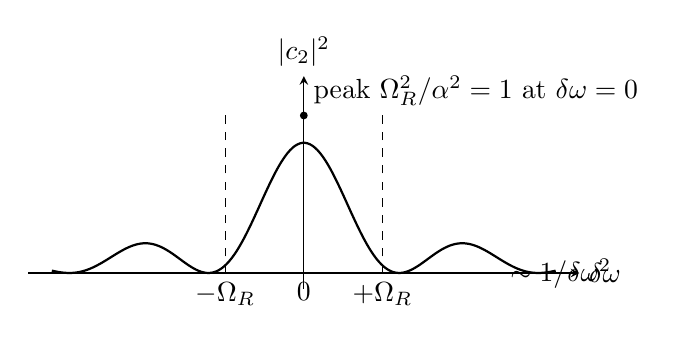
\begin{tikzpicture}[>=stealth, scale=1.0]
\draw[->] (-3.5,0) -- (3.5,0) node[right] {$\delta\omega$};
\draw[->] (0,-0.2) -- (0,2.5) node[above] {$|c_2|^2$};
\node[below] at (0,0) {$0$};
% Lorentzian-like central + side lobes
\draw[thick,domain=-3.2:3.2,samples=200,smooth] plot (\x,{2*sin(deg(0.5*sqrt(1+\x*\x)*4))*sin(deg(0.5*sqrt(1+\x*\x)*4))/(1+\x*\x)});
\node[circle,fill,inner sep=1pt] (P) at (0,2) {};
\node[above right] at (P) {peak $\Omega_R^2/\alpha^2 = 1$ at $\delta\omega=0$};
\draw[dashed] (-1,0) node[below]{$-\Omega_R$} -- (-1,2);
\draw[dashed] (1,0) node[below]{$+\Omega_R$} -- (1,2);
\node[below right] at (2.5,0.3) {$\sim 1/\delta\omega^2$};
\end{tikzpicture}
\end{center}

Central peak height 1 (full transfer at resonance, fixed $t$ chosen so $\sin^2(\Omega_R t/2)=1$); side lobes decay $\sim 1/\delta\omega^2$, half-width $\sim\Omega_R$.

\subsection*{(d) Three-level: $c_2(t)$ to leading order}

Take initial conditions $c_1(0)=1$, $c_2(0)=c_3(0)=0$; in weak light keep $c_1\approx 1$ and $c_3\approx 0$:
\[
\dot c_2 \approx -i\Omega_R\cos\omega t\,e^{i\omega_0 t}.
\]
Expand $\cos\omega t$:
\[
\dot c_2 \approx -i\tfrac{\Omega_R}{2}\bigl[e^{i(\omega_0+\omega)t}+e^{i(\omega_0-\omega)t}\bigr].
\]
Apply RWA (drop $e^{i(\omega_0+\omega)t}$, keep $e^{-i\delta\omega t}$):
\[
\dot c_2 \approx -i\tfrac{\Omega_R}{2}\,e^{-i\delta\omega t}.
\]
Integrate from $0$ to $t$ with $c_2(0)=0$:
\[
c_2(t) = -i\tfrac{\Omega_R}{2}\int_0^t e^{-i\delta\omega t'}\,\de t'.
\]
Evaluate the integral:
\[
c_2(t) = -i\tfrac{\Omega_R}{2}\cdot\frac{1-e^{-i\delta\omega t}}{i\delta\omega}.
\]
Cancel the $i$'s:
\[
\boxed{\;c_2(t) \approx -\frac{\Omega_R}{2\delta\omega}\bigl(1-e^{-i\delta\omega t}\bigr).\;}
\]
Amplitude $\sim\Omega_R/\delta\omega\ll 1$ when $\delta\omega\gg\Omega_R$: the off-resonant intermediate level is only weakly admixed.

\subsection*{(e) Effective two-photon Rabi flopping for $c_3$}

Define single-photon detunings $\delta\omega\equiv\omega-\omega_0$ and $\omega-\phi_0$; the two-photon detuning is $\Delta\omega = \omega_0+\phi_0-2\omega$. Near two-photon resonance $\Delta\omega\to 0$, so $\delta\omega\approx \phi_0-\omega$; both intermediate detunings are large compared to $\Omega_R,\Phi_R$.

Expand $\cos\omega t$ in the $\dot c_2$ equation:
\[
\dot c_2 = -i\tfrac{\Omega_R}{2}\bigl[e^{i(\omega_0+\omega)t}+e^{i(\omega_0-\omega)t}\bigr]c_1 -i\tfrac{\Phi_R}{2}\bigl[e^{-i(\phi_0-\omega)t}+e^{-i(\phi_0+\omega)t}\bigr]c_3.
\]
Drop the fast-rotating terms $e^{\pm i(\omega_0+\omega)t}$, $e^{-i(\phi_0+\omega)t}$:
\[
\dot c_2 = -i\tfrac{\Omega_R}{2}e^{-i\delta\omega t}c_1 - i\tfrac{\Phi_R}{2}e^{-i(\phi_0-\omega)t}c_3.
\]
Adiabatically eliminate $c_2$: with $c_1, c_3$ slow, $c_2$ follows the driving. Take the ansatz $c_2 = a\,e^{-i\delta\omega t}c_1 + b\,e^{-i(\phi_0-\omega)t}c_3$ and demand $\dot c_2$ match:
\[
-i\delta\omega\,a\,e^{-i\delta\omega t}c_1 -i(\phi_0-\omega)\,b\,e^{-i(\phi_0-\omega)t}c_3 = -i\tfrac{\Omega_R}{2}e^{-i\delta\omega t}c_1 - i\tfrac{\Phi_R}{2}e^{-i(\phi_0-\omega)t}c_3.
\]
Match coefficients of $e^{-i\delta\omega t}c_1$:
\[
a = \frac{\Omega_R}{2\delta\omega}.
\]
Match coefficients of $e^{-i(\phi_0-\omega)t}c_3$:
\[
b = \frac{\Phi_R}{2(\phi_0-\omega)}.
\]
Assemble $c_2$:
\[
c_2 \approx \frac{\Omega_R}{2\delta\omega}\,e^{-i\delta\omega t}c_1 + \frac{\Phi_R}{2(\phi_0-\omega)}\,e^{-i(\phi_0-\omega)t}c_3.
\]
Take the RWA $\dot c_3$ equation:
\[
\dot c_3 = -i\tfrac{\Phi_R}{2}\,e^{i(\phi_0-\omega)t}c_2.
\]
Substitute $c_2$:
\[
\dot c_3 = -i\tfrac{\Phi_R}{2}\Bigl[\tfrac{\Omega_R}{2\delta\omega}e^{i(\phi_0-\omega-\delta\omega)t}c_1 + \tfrac{\Phi_R}{2(\phi_0-\omega)}c_3\Bigr].
\]
Combine exponents using $(\phi_0-\omega)-\delta\omega = \omega_0+\phi_0-2\omega = \Delta\omega$:
\[
\dot c_3 = -i\,\tfrac{\Omega_R\Phi_R}{4\delta\omega}\,e^{i\Delta\omega t}\,c_1 - i\,\tfrac{\Phi_R^2}{4(\phi_0-\omega)}\,c_3.
\]
Identify the AC-Stark light shift on level 3:
\[
\delta_3 = \frac{\Phi_R^2}{4(\phi_0-\omega)}.
\]
Repeat the elimination for $\dot c_1 = -i(\Omega_R/2)e^{i\delta\omega t}c_2$:
\[
\dot c_1 = -i\,\tfrac{\Omega_R^2}{4\delta\omega}\,c_1 - i\,\tfrac{\Omega_R\Phi_R}{4(\phi_0-\omega)}\,e^{-i\Delta\omega t}c_3.
\]
Identify the AC-Stark shift on level 1:
\[
\delta_1 = \frac{\Omega_R^2}{4\delta\omega}.
\]
Near two-photon resonance set $\delta\omega\approx \phi_0-\omega$ in the off-diagonal terms and define the effective two-photon Rabi frequency:
\[
\Omega_\text{eff} \equiv \frac{\Omega_R\Phi_R}{2\,\delta\omega}.
\]
The reduced two-level system reads:
\[
\dot c_1 = -i\delta_1 c_1 - i\tfrac{\Omega_\text{eff}}{2}e^{-i\Delta\omega t}c_3,
\]
\[
\dot c_3 = -i\delta_3 c_3 - i\tfrac{\Omega_\text{eff}}{2}e^{i\Delta\omega t}c_1.
\]
Absorb the diagonal shifts into a modified detuning $\Delta\omega' = \Delta\omega + \delta_3 - \delta_1$, then apply the result of part (b):
\[
\boxed{\;|c_3(t)|^2 = \frac{\Omega_\text{eff}^2}{\beta^2}\sin^2(\beta t/2),\quad
\Omega_\text{eff}=\frac{\Omega_R\Phi_R}{2\,\delta\omega},\quad
\beta = \sqrt{\Omega_\text{eff}^2 + (\Delta\omega + \delta_3-\delta_1)^2}.\;}
\]
(Often the AC-Stark shifts are absorbed into a redefined two-photon detuning, leaving $\beta=\sqrt{\Omega_\text{eff}^2+\Delta\omega^2}$.)

%==================================================================
\section*{Question 4 --- Einstein coefficients and astrophysical lasers}

\subsection*{(a) Einstein $A$, $B_{ul}$, $B_{lu}$}

Three processes between levels $u$ (energy $E_u$) and $l$ ($E_l$), $h\nu_0=E_u-E_l$, in radiation field of spectral energy density $\rho(\nu)$:
\begin{itemize}
\item \textbf{Spontaneous emission}, $A_{ul}$: rate per atom $A_{ul}$. Power emitted: $N_u A_{ul} h\nu_0$.
\item \textbf{Stimulated emission}, $B_{ul}$: rate per atom $B_{ul}\rho(\nu_0)$. Power emitted: $N_u B_{ul}\rho(\nu_0) h\nu_0$.
\item \textbf{Absorption}, $B_{lu}$: rate per atom $B_{lu}\rho(\nu_0)$. Power absorbed: $N_l B_{lu}\rho(\nu_0) h\nu_0$.
\end{itemize}
Detailed balance (thermal, Planck): $g_l B_{lu}=g_u B_{ul}$ and $A_{ul}/B_{ul}=8\pi h\nu_0^3/c^3$.

\subsection*{(b) $I_S\propto\nu_0^3$ for radiative-only upper level}

Write the gain cross section at line centre (Lorentzian, $\nu_L\approx\nu_0$):
\[
\sigma_{ul}(\nu_0) = \frac{\lambda_0^2}{8\pi}\,A_{ul}\,\phi(\nu_0),\qquad \phi(\nu_0)=\frac{2}{\pi\Delta\nu}.
\]
Insert $\phi(\nu_0)$:
\[
\sigma_{ul}(\nu_0) = \frac{\lambda_0^2 A_{ul}}{4\pi^2\Delta\nu}.
\]
Upper level radiatively dominated: $\tau_u = 1/A_{ul}$, equivalently $\tau_u A_{ul} = 1$.

Factor $(g_u/g_l)\tau_l$ in the bracket of $I_S$:
\[
\tau_u + \tfrac{g_u}{g_l}\tau_l - \tfrac{g_u}{g_l}\tau_u\tau_l A_{ul}
= \tau_u + \tfrac{g_u}{g_l}\tau_l(1-\tau_u A_{ul}).
\]
Apply $\tau_u A_{ul}=1$:
\[
\tau_u + \tfrac{g_u}{g_l}\tau_l(1-1) = \tau_u = \frac{1}{A_{ul}}.
\]
Insert into the saturation formula:
\[
I_S = \frac{h\nu_L}{\sigma_{ul}}\bigl(1/A_{ul}\bigr)^{-1} = \frac{h\nu_L A_{ul}}{\sigma_{ul}}.
\]
Substitute $\sigma_{ul}=\lambda_0^2 A_{ul}/(4\pi^2\Delta\nu)$:
\[
I_S = h\nu_L A_{ul}\cdot\frac{4\pi^2\Delta\nu}{\lambda_0^2 A_{ul}}.
\]
Cancel $A_{ul}$:
\[
I_S = \frac{4\pi^2 h\nu_L\Delta\nu}{\lambda_0^2}.
\]
Use $\lambda_0 = c/\nu_0$, so $\lambda_0^2 = c^2/\nu_0^2$:
\[
I_S = \frac{4\pi^2 h\nu_L\nu_0^2\Delta\nu}{c^2}.
\]
Set $\nu_L\approx\nu_0$:
\[
\boxed{\;I_S = \frac{4\pi^2 h\,\nu_0^3\,\Delta\nu}{c^2}\propto \nu_0^3.\;}
\]

\subsection*{(c) Spontaneous-emission photon rate from the seed region}

Compute the total spontaneous rate from the cylinder (volume $\pi d^2\ell/4$, density $N_u$):
\[
\dot N_\gamma^\text{spon} = \frac{\pi d^2}{4}\,\ell\,N_u\,A_{ul}.
\]
Use $N_u\approx N^*$ for a large initial inversion ($N_l\ll N_u$):
\[
\dot N_\gamma^\text{spon} = \frac{\pi d^2}{4}\,N^*\ell\,A_{ul}.
\]
Insert the gain-length condition $\sigma_{ul}N^*\ell = 1$ as $N^*\ell = 1/\sigma_{ul}$:
\[
\dot N_\gamma^\text{spon} = \frac{\pi d^2}{4}\,\frac{A_{ul}}{\sigma_{ul}}.
\]
From part (b), $I_S = h\nu_L A_{ul}/\sigma_{ul}$, hence $A_{ul}/\sigma_{ul} = I_S/(h\nu_0)$:
\[
\boxed{\;\dot N_\gamma^\text{spon} = \frac{\pi d^2 I_S}{4 h\nu_0}.\;}
\]

\subsection*{(d) Minimum length to reach saturation}

In the unsaturated regime $N^*$ is constant. Write the gain equation:
\[
\frac{\de I}{\de z} = \sigma_{ul}N^*\,I.
\]
Use $\sigma_{ul}N^*\ell = 1$:
\[
\frac{\de I}{\de z} = \frac{I}{\ell}.
\]
Integrate with seed intensity $I_0$ at $z=0$:
\[
I(z) = I_0\,e^{z/\ell}.
\]
Estimate the seed intensity: spontaneous power forward $=\eta\cdot h\nu_0 A_{ul}N_u\cdot(\pi d^2\ell/4)$ over beam area $\pi d^2/4$:
\[
I_0 = \eta\,h\nu_0\,A_{ul}\,N_u\,\ell.
\]
Saturation occurs when $I(L_S)=I_S$:
\[
I_S = I_0\,e^{L_S/\ell}.
\]
Take the logarithm:
\[
\frac{L_S}{\ell} = \ln\!\left(\frac{I_S}{I_0}\right).
\]
Substitute $I_0$ and split the log:
\[
\frac{L_S}{\ell} = \ln(1/\eta) + \ln\!\left(\frac{I_S}{h\nu_0 A_{ul}N_u\ell}\right).
\]
Use $I_S = h\nu_0 A_{ul}/\sigma_{ul}$ (part b) in the second log:
\[
\frac{I_S}{h\nu_0 A_{ul}N_u\ell} = \frac{1}{\sigma_{ul}N_u\ell}.
\]
Apply $\sigma_{ul} N^*\ell=1$ with $N^*\approx N_u$:
\[
\frac{1}{\sigma_{ul}N_u\ell} = 1.
\]
The second logarithm vanishes:
\[
\frac{L_S}{\ell} = \ln(1/\eta).
\]
Use $\ell = 1/(\sigma_{ul}N_u) = I_S/(h\nu_0 A_{ul}N_u)$:
\[
\boxed{\;L_S \simeq \frac{I_S}{h\nu_0\,A_{ul}\,N_u}\,\ln(1/\eta).\;}
\]

\subsection*{(e) Estimate of $\eta$}

Photons are emitted isotropically from the seed region. The fraction reaching the far end is the geometric ratio of its solid angle:
\[
\eta \sim \frac{\Delta\Omega}{4\pi} = \frac{\pi d^2/4}{4\pi L^2}.
\]
Simplify:
\[
\boxed{\;\eta \sim \frac{d^2}{16\,L^2}.\;}
\]
For $d\ll L$ this is small but enters $L_S$ only logarithmically: $\ln(1/\eta)\sim 2\ln(4L/d)$.

\end{document}
